
%% INTRODUCTION

%% ------- Text from GECON'15  %% USE CASES
When cloud applications are deployed within community networks, 
in many cases connectivity external to the community network is important. 
Even when cloud applications are deployed using resources solely available within community networks, 
they require connection to the Internet for functioning.
In the basic case, cloud applications may want to backup or synchronise data with servers external to the community network,
or require fetching data for operating the service, for instance a video-on-demand service may download fresh content.
Also, a service available in multiple community networks requires access at the gateways for exchanging data, and gateways in this case act to federate the community networks.
Applications for Internet of Things and smart cities involve collecting data from the sensors, 
which may have to be shared with servers outside the community network for data analysis.
For the case of edge clouds, the servers residing within the community networks, acting as nano data centres, require connectivity to the data centres.
In all these situations, the applications deployed on servers within the community network require bandwidth at the gateways 
with quality-of-service (QoS) guarantees to connect to the Internet, 
though their requirements for robustness, waiting time, throughput, and prioritising network traffic, may vary for different scenarios.
Figure~\ref{fig__external_bandwith_mesh_network} shows how such an edge cloud can be deployed within a community network.
The servers are present at different locations, 
either caching content for media-rich applications or performing computation locally for time-critical applications.
These servers require connection to the data centres through the Internet,
for which they rely on the gateway providers available in the community network~\cite{Baig2015Guifi}.

%% FIGURE
\begin{figure}[tbp]
	\centering
	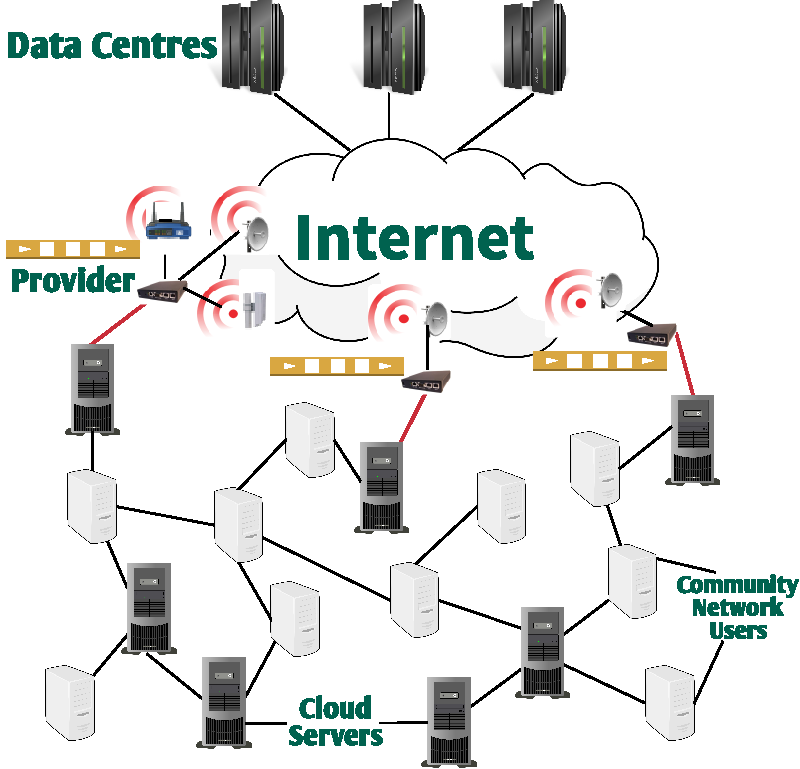
\includegraphics[width=0.75\columnwidth,keepaspectratio]{network}
	\caption[Users connected to the service provider's gateway]{Users connected to the service provider's gateway in a community network}
	\label{fig__external_bandwith_mesh_network}
\end{figure} 

%% ------- Text from INFOCOM/ICDCS Submission
%Community networks are based on the principle of reciprocal sharing and most of their users are moved by altruistic principles. 
Community networks, as any other human organisation, are not immune to overuse, free riding, or under-provisioning, 
specially in scenarios where users may have motivations to compete for scarce resources. 
In this chapter, we consider the concrete problem of bandwidth reservation on the gateways that connect the community network to the Internet. 
In particular, we consider that, as in most community networks, the subset of users that offer gateway services to the Internet is smaller than the complete set of users. 
Users that are not at the gateways may be interested in reserving bandwidth in these gateways for Internet access.
If the available bandwidth at each gateway is not enough to satisfy the demand, 
one needs to implement some arbitration mechanism that optimally and fairly allocate resources, 
Note that we are not considering the bandwidth on the links internal to the community network,
because network is operated in a shared manner, 
and this bandwidth is collectively owned by the community.


%% ------- Text from INFOCOM
Most of the auction-based game theoretical approaches in literature, 
as we discussed in \cref{sec__resource_regulation}, 
assume that the auctioneer is trusted.
This is an unreasonable assumption in community networks, where no entity can be trusted,
and even if such entity existed, it would be a bottleneck. 
Thus, there is a substantial gap that needs to be bridged to apply these results in community networks.
In this chapter, our aim is to address this gap by by proposing a framework of 
distributed protocols that allows multiple resource providers 
in a community network to simulate the role of the auctioneer.
Such simulation raises significant challenges both from the 
theoretical and practical points of view. 
From the theoretical perspective, 
although there is a vast literature of distributed fault-tolerant algorithms, 
with very few exceptions (for instance,~\cite{Abraham2013}), 
these works do not consider rational behaviour. From the practical 
perspective, the distribution of the auctioneer may incur 
additional overhead. Our proposal addresses both concerns. First, 
we prove that our distributed simulations are sound from a game 
theoretical perspective. Specifically, we show that the 
simulations are $k$-resilient (ex post) equilibria~\cite{Abraham2013}, i.e., 
Nash equilibria resilient to asynchrony and coalitions of providers 
of size at most $k$. 
Second, our protocols leverage the distributed nature of the 
resulting virtual trusted entity to parallelise the resource 
provisioning algorithm, compensating for the additional costs
imposed by coordination. 
We have implemented a prototype of our
protocols and evaluated the resulting system in a real community network. 

Even though in our example we only focus on bandwidth
reservation, the fundamental problems at hand are general and emerge
every time shared resources need to be allocated to users in a set of
providers, such as for allocation of processing and memory resources
as virtual machines in public clouds~\cite{Zhang2015Truthful},
assignment of frequencies in secondary wireless spectrum
markets~\cite{Zhou2008}, and resource scheduling in grid and cloud
infrastructures\cite{Lai2004}.

In summary, our main contributions in this chapter are the following:

\begin{itemize}

\item We propose a framework for devising distributed protocols executed among service providers that correctly simulate the
auctioneer in a family of resource allocation auctions.

\item We show that every implementation of the framework is a $k$-resilient (ex post) equilibrium.
These implementations also tolerate users that send invalid bids.

\item We show that it is possible to leverage the distributed nature of our framework to parallelise implementations,
mitigating scalability issues of purely centralised solutions.

\item We implement instances of the framework and report the results from its deployment on the actual Guifi.net nodes.

\end{itemize}


\vspace{0.3mm}
The rest of the chapter is organised as follows.
First, we discuss the motivation for a truthful and trusted resource allocation mechanism in \Cref{sec__truthful_pricing_introduction}.
Next, we provide the system model in \Cref{sec__dist_auctioneer_model}.
We present the framework for simulating the auctioneer in \Cref{sec__dist_auctioneer_design}, 
and we illustrate its applicability to the execution
of two different auction mechanisms,
with different computational properties, in \Cref{sec__dist_auctioneer_instances}.
We discuss results from the experiments using a prototype for distributed auctioneer in \Cref{sec__dist_auctioneer_evaluation}.
%We summarise our findings in \Cref{sec__dist_auctioneer_conclusion}, 
%and include the proofs of the main theorems in \Cref{sec__dist_auctioneer_proofs}.

